\chapter{Methods on operators}\label{Sec:SparcoMetaOp} % Operator manipulation

All \sparco{} operators provide routines for multiplying vectors by
itself and its conjugate. The real power of the operator toolbox is
the ease with which basic operators (see Section
\ref{Sec:SparcoOperators}) can be combined into more powerful
operators, which themselves can be combined into yet more powerful
operators. In this section we discuss the type of operations can be
applied to all \sparco{} operators. All operations discussed in this
section are implemented using underlying meta-operators. Pointers to
these operators are given at the end of each section, where
relevant. In the cases where the meta-operators provide more extensive
possibilities, they are described in more detail below the basic use.

We denote by $A$--$D$ arbitrary \sparco{} operators and by $M$ any
matrix. All operator and matrix are assumed to have appropriate
dimensions that can vary line per line. Most operations described in
this section are meaningful only when applied to linear operators; see
\ref{Sec:NonLinearOperators} for more details.

\section{Multiplication}

Multiplication by operators is the most elementary operation in
\sparco. In its simplest form we have operator-vector products such
as:
\begin{codeblock}
y = A * x;
z = B * y;
n = m'* C;  % Evaluated as $n = (C^Hm)^H$
\end{codeblock}
This will evaluate the application of $A$ on $x$, and then $B$ to
$y$. In both cases the result will be an explicit vector of real or
complex numbers. An equivalent approach is to first create a new
operator $C$ representing the product $B\cdot A$, and then apply this
to $x$ to immediately get vector $z$:
\begin{codeblock}
C = B * A;  % Construct compound operator
z = C * x;  % Evaluate $z = BAx$
\end{codeblock}
Although \sparco{} operators are expected to support only
multiplication of vectors, it is possible to write operator-matrix
multiplications. However, it should be kept in mind that this is
implemented as a series of operator-vector multiplications.
\begin{codeblock}
N = C * M;
N = M * C;  % Evaluated as $N = (C^HM^H)^H$
\end{codeblock}
A special case of multiplication is multiplication by
scalars. Generally, this will give a new operator scaled by that
quantity;
\begin{codeblock}
C = 3 * A;  % Construct compound operator $C = 3A$
C = A * 3;
\end{codeblock}
One notable exception is when the corresponding dimension of the
operator is one. In that case we have a valid matrix-vector product
which results in a numeric solution. In other words, matrix-vector
products take precedence over scalar multiplication. In such cases it
is still possible to scale the operator, either by changing the order
(as shown above) or by directly setting the \mlcmd{.scalar} property
of the operator (for more details see Section \ref{Sec:SparcoOpFields}).
Two remaining special cases are multiplication by $\pm 1$, indicated
by the unary plus and minus operations
\begin{codeblock}
C = -A;
B = +A;
\end{codeblock}
This works regardless of the dimensions of the operator. Note that
elementwise multiplication using \mlcmd{.*} is not supported as this
would require the explicit matrix underlying the operator to be known.

In the evaluation and comparison of algorithms it is often useful to
know how many multiplications have been performed using a given
operator. To facilitate these kind of measurements it is possible to
associate a counter variable to each operator. This is discussed in
detail in Section \ref{Sec:SparcoCounters}.

\vspace*{1em}
\coderefs{\mlcmd{opFoG}}

\section{Transposition and conjugation}

As mentioned in the introduction, each \sparco{} operator implements
multiplication by itself and its conjugate. Using \matlab's transpose
operator \mlcmd{'} returns a new operator in which these two modes are
switched.
\begin{codeblock}
B = A';
x = A'* y;
x = B * y; % Identical result as previous line
\end{codeblock}
When using transposes within calculations these new operators are
discarded as soon as the multiplication has been done. Since
transposes in \sparco{} are simple book keeping operations, they are
essentially free; no underlying matrices are actually transposed.
%
The transpose of a complex operator, rather than its conjugate, can be
formed using the \mlcmd{.'} operator. This is implemented as the
elementwise conjugate (see \mlcmd{conj} in Section
\ref{Sec:SparcoConj}) of the conjugate;
\begin{codeblock}
A = C.'; % Transpose of complex operator, $C^T = \overline{(C^H)}$
\end{codeblock}
Note that in this case a single multiplication of a complex vector by
$A$ requires two multiplications by $C^H$ due to the implementation of
the \mlcmd{conj} operation. When applied to a real operator, the
\mlcmd{.'} operation reduces to the standard \mlcmd{'} operation.


\section{Addition and subtraction}

The next elementary operation is the addition and subtraction of
operators. In its simplest for we add two or more operators;
\begin{codeblock}
x = (B + C + D) * y;
A = B + C + D;
x = A * y;           % Equivalent to first statement
\end{codeblock}
When \sparco{} encounters the sum of an operator with a matrix or some
class object that implements the multiplication and size operators, it
will first wrap that entity to a \sparco{} operator using the
\mlcmd{opMatrix} command (see Section \ref{Sec:SparcoOpMatrix}). This
allows us to write
\begin{codeblock}
C = A + M;  % Addition of operator and matrix
C = M + A;  % Addition of matrix and operator
\end{codeblock}
Addition of scalars to an operator is interpreted as an elementwise
addition, just like it is done for matrices. In order to make this
work we first create a new operator of appropriate size, consisting of
only ones (see Section \ref{Sec:SparcoOpOnes}), and premultiply that
with the scalar. The following two statements are therefore equivalent
\begin{codeblock}
A = B + 3;
A = B + 3*opOnes(size(B));
\end{codeblock}
Subtraction is implemented by scalar multiplication combined with
addition.
\begin{codeblock}
A = B - C;
A = B + (-C);
\end{codeblock}
Unfortunately, \sparco{} can only provide a limited amount of
simplification of operators. This means that in the following case, no
simplification is done;
\begin{codeblock}
A = B + 3 - 2; % Not simplified, A = B + 3 - 2;
A = B + C - C; % Not simplified
\end{codeblock}

\coderefs{\mlcmd{opSum}}

\section{Operator information}\label{Sec:SparcoDisp}
\label{Sec:SparcoIsReal}

Before we proceed with more advanced operator manipulations, let us
briefly look at some ways of querying operator information. This kind
of information is useful when developing algorithms and also enable us
to explain how certain operator manipulations work.

The most elementary property of each operator is its size, and it can
be queried using the \mlcmd{size} command. The use of this command is
best illustrated using a number of examples based on a $3\times 6$
operator \mlcmd{A}:
\begin{codeblock}
[m,n] = size(A);    % Gives m = 3, n = 6;
m = size(A,1);      % Gives m = 3;
n = size(A,2);      % Gives n = 6;
o = size(A,3);      % Gives o = 1;
\end{codeblock}
Note that the first two dimensions give the number of rows and columns
respectively. All higher dimensions have size one by definition. To
check if an operator is empty we can use \mlcmd{isempty}:
\begin{codeblock}
if isempty(A)
   error('Operator A cannot be empty');
end
\end{codeblock}
An operator is considered empty if either its number of rows or its
number of columns is zero; a $0\times 6$ operator, albeit of limited
use, is perfectly valid and can be applied to vectors of corresponding
size.

When working interactively from the Matlab command line it is often
more convenient to display the operator by typing its name, or using
the \mlcmd{disp} and \mlcmd{whos} commands. For the following example
we assume that operator $A$ is the operator representation of a
$3\times 6$ matrix (see Section \ref{Sec:SparcoOpMatrix})
\begin{codeblock}
>> A
A is a linear Sparco operator of size 3 x 6
         Matrix(3,6)
>> disp(A)
ans is a linear Sparco operator of size 3 x 6
         Matrix(3,6)
>> whos A
  Name      Size            Bytes  Class       Attributes

  A         3x6              1309  sparcoOp              
\end{codeblock}
The first two commands also provide information about the construction
of the operator:
\begin{codeblock}
>> B = A'*A
B is a linear Sparco operator of size 6 x 6
         (Matrix(6,3))' * Matrix(3,6)
\end{codeblock}

At times, for example during debugging or when using codes not
compatible with \spot{}, it is desirable to have access to the matrix
form underlying an operator. This can be done identically using the
\mlcmd{double}, or \mlcmd{full} commands:
\begin{codeblock}
>> A = opDCT(4);
>> double(A)
ans =
    0.5000    0.5000    0.5000    0.5000
    0.6533    0.2706   -0.2706   -0.6533
    0.5000   -0.5000   -0.5000    0.5000
    0.2706   -0.6533    0.6533   -0.2706
\end{codeblock}
This explicit form is obtained though multiplication by the identity
matrix. As such, it can be quite an expensive operator. When the
number of rows is much smaller than the number of columns it may be
faster to use \mlcmd{double(A')'} instead of \mlcmd{double(A)}.

Finally, the command \mlcmd{isreal} can be used to check if the
operator is real or complex (see Section \ref{Sec:SparcoRealComplex}
for more details on this).  More advanced commands such as
\mlcmd{isfield}, \mlcmd{set}, \mlcmd{get}, and cell indexing will be
discussed in Section \ref{Sec:SparcoImplementation}, which deals with
the implementation of \spot{}.

\section{Dictionaries and arrays}

The original motivation for developing \sparco{} was the concatenation
of operators to form a dictionary. This can now be achieved simply by
writing 
\begin{codeblock}
A = [B,C,M]; % or
A = [B C M];
\end{codeblock}
Note that explicit matrices and classes can be mixed with \sparco{}
operators, provided they are all compatible in size. Like in operator
addition \sparco{} automatically converts these entities to \sparco{}
operators. Vertical concatenation is done likewise by typing
\begin{codeblock}
A = [B;C;M]; % or
A = [B
     C
     M];
\end{codeblock}
With the specification of these two operations, \matlab{} automatically
converts arrays of operators into a vertical concatenation of
dictionaries: 
\begin{codeblock}
A = [B C; C' M]; % or
A = [B   C
     C'  M];     % both represent A = [[B,C];[C',M]];
\end{codeblock}

\coderefs{\mlcmd{opDictionary}, \mlcmd{opStack}}

\section{Block diagonal operators}

Analogous to matrices of operators it is possible to construct block
diagonal operators of operators, using the \mlcmd{diag} and
\mlcmd{blkdiag} commands. Both commands take a list of operators and
matrices to create the desired operator:
\begin{codeblock}
D = diag(A,B,C,M);
D = blkdiag(A,B,C,M);
\end{codeblock}
There is no restriction on the dimension of each operator. This means
that the resulting operator need not necessarily be square:
\begin{center}
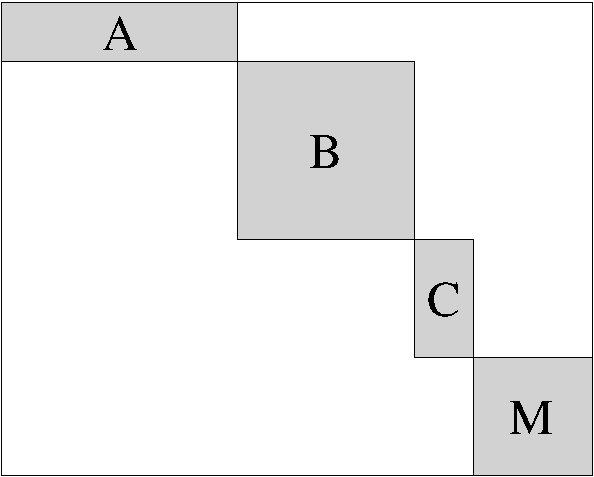
\includegraphics[width=4cm]{./FigSparcoBlockDiag1}
\end{center}
Any matrix or class object that is encountered is automatically
converted into a \spot{} operator. The commands \mlcmd{diag} and
\mlcmd{blkdiag} differ in the way in which explicit vectors are dealt
with in the argument list. Whereas \mlcmd{blkdiag} treats vectors just
like any other matrix, \mlcmd{diag} interprets the vector as the
diagonal entries of a matrix, which is then added as a block. This
behavior is illustrated in the following example
\begin{codeblock}
> D = diag(opDCT(2),ones(2,1)); double(D)
ans =
    0.7071    0.7071         0         0
    0.7071   -0.7071         0         0
         0         0    1.0000         0
         0         0         0    1.0000
> D = blkdiag(opDCT(2),ones(2,1)); double(D)
ans =
    0.7071    0.7071         0
    0.7071   -0.7071         0
         0         0    1.0000
         0         0    1.0000
\end{codeblock}
For more powerful constructions, including horizontal or vertical
overlap of operators the underlying command \mlcmd{opBlockDiag} has to
be called directly.

In section \ref{Sec:SparcoDisp} we illustrated the \mlcmd{isempty}
command on an empty $0\times 6$ operators. Such operators, although
seemingly useless, can come in handy when constructing block-diagonal
operators that require horizontal or vertical padding between certain
blocks.

\paragraph{Advanced interface} The block-diagonal operator can be
invoked in two different ways:
\begin{codeblock}
op = opBlockDiag([weight],op1,...,opn,[overlap]);
op = opBlockDiag([weight],op,[overlap]);
\end{codeblock}
In the first mode, a block-diagonal operator is formed using operators
$1,\ldots,n$, with weights set to
\mlcmd{weight(1)},$\ldots$,\mlcmd{weight(n)}, and a horizontal or
vertical overlap given by parameter \mlcmd{overlap}. Arguments in the
operator list that are not \spot{} operators are automatically
converted using the \mlcmd{opMatrix} command. The sign of the overlap
parameter determines whether overlap should be horizontal or vertical:
\begin{center}
\begin{tabular}{ccc}
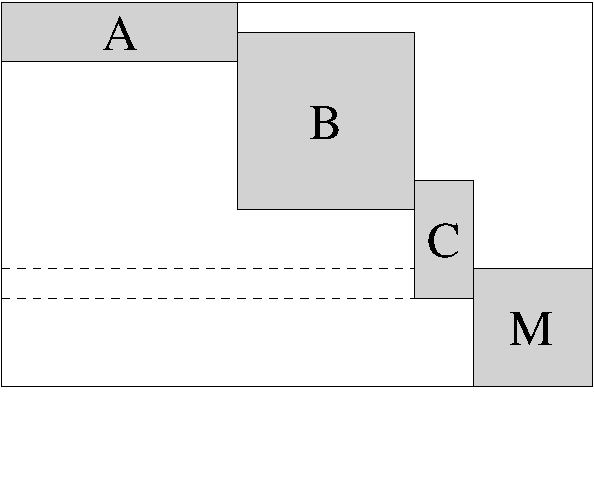
\includegraphics[height=32mm]{./FigSparcoBlockDiag2} & &
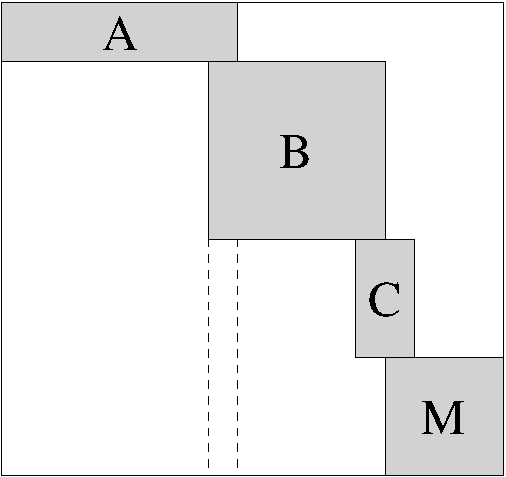
\includegraphics[height=32mm]{./FigSparcoBlockDiag3} \\
Vertical: overlap $>0$ & &
Horizontal: overlap $< 0$
\end{tabular}
\end{center}
The weight and overlap parameters are optional and are set to
\mlcmd{[]}, respectively \mlcmd{0} by default. When the first argument
to \mlcmd{opBlockDiag} is numerical it is interpreted as a weight
parameter, and likewise for the last argument and overlap. Thus,
special care has to be taken when either parameter is omitted while
the first (resp. last) operator is an explicit vector or matrix. This
is best avoided by explicitly specifying the default arguments
whenever ambiguity can arise.

The second mode, with only a single operator specified, can be used to
replicate the given operator. When the vectorized weight parameter,
\mlcmd{weight(:)} is not a scalar its length gives the number of
replications of the operator, each with its corresponding weight. A
scalar weight simply gives the replication count and implies a weight
of one on each operator. Anti-diagonal operators can be obtained by
setting the overlap to twice the dimension of the operator (this also
works in the first mode). An illustration of this with \mlcmd{A} a
$2\times 3$ \sparco{} is given by
\begin{center}
\begin{tabular}{ccc}
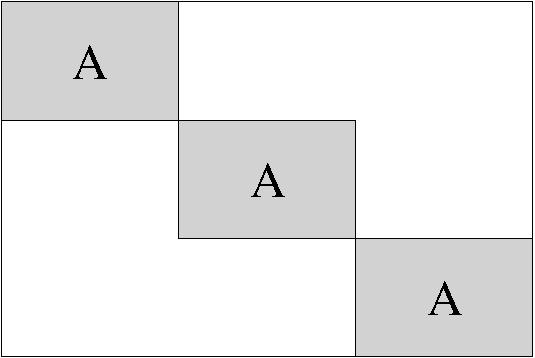
\includegraphics[width=0.3\textwidth]{./FigSparcoBlockDiag4} &
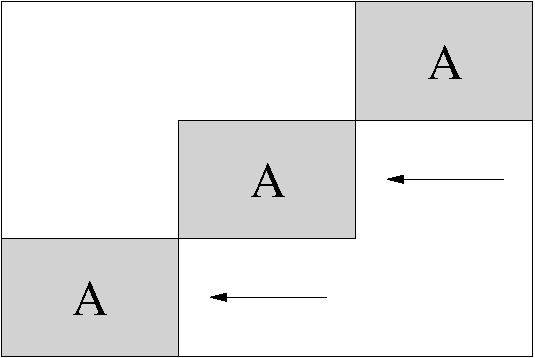
\includegraphics[width=0.3\textwidth]{./FigSparcoBlockDiag5} &
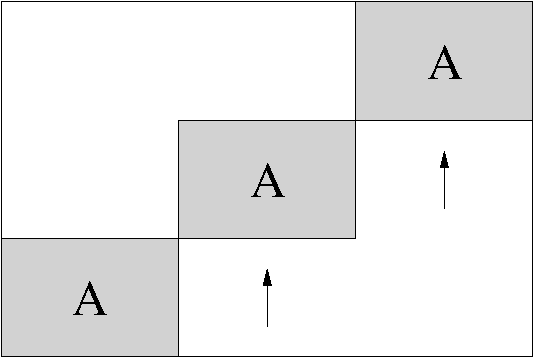
\includegraphics[width=0.3\textwidth]{./FigSparcoBlockDiag6} \\
\mlcmd{opBlockDiag(3,A,0)} &
\mlcmd{opBlockDiag(3,A,-6)} &
\mlcmd{opBlockDiag(3,A,4)}
\end{tabular}
\end{center}


\paragraph{Example}

The block-diagonal operator can be very useful in constructing
windowed Fourier transformations.

\vspace*{1em}
\coderefs{\mlcmd{opBlockDiag}}

\section{Kronecker products}

The \mlcmd{kron} operator allows the creation of Kronecker products
between operators. Unlike \matlab's built-in \mlcmd{kron} function,
the \mlcmd{kron} product in \sparco{} can take an arbitrary number of
arguments. Hence to construct $D = A \otimes B \otimes C$ we can type
\begin{codeblock}
D = kron(A,B,C)
\end{codeblock}
Needless to say, Kronecker products can increase quickly in
computational complexity. Given a set of operators of size $m_i\times
n_i$, $i=1,\ldots,k$, let $m = \prod m_i$, and $n = \prod n_i$. Then,
application of the Kronecker product will require $n / n_i$
multiplications with each operator $i$, and likewise $m / m_i$
products in transpose mode.

\paragraph{Example}
Kronecker products can be useful when operating on high dimensional
data represented in vectorized form. For example, when $x$ represents
a data volume of dimensions $l\times m\times n$.  To create an
operator that applies a one-dimensional Fourier transformation on
vectors along the second dimension, we can simply write
\begin{codeblock}
op = kron(opEye(n),opFFT(m),opEye(l))
\end{codeblock}
Likewise, the block diagonal matrix of three operators $A$, given in
the previous section, could have been created using the Kronecker
product: \mlcmd{kron(opEye(3),A)}. This latter construction was
found to outperform the block diagonal operator consisting of even a
moderate number of identical blocks.

\vspace*{1em}
\coderefs{\mlcmd{opKron}}

\section{Subset assignment and reference}

For certain applications we may be interested only in applying part
of an operator. This can be done by creating new operators that are
restrictions of existing operators. Restriction can be done in terms
of rows, columns, a combination of rows and columns, and in terms of
individual elements of the underlying matrix. Like in matrices, this
is done by indexing using brackets. 
\begin{codeblock}
A = B(3:5,:);     % Extract rows 3-5
A = C(:,4:6);     % Extract columns 4-6
A = D(3:5,4:6);   % Extract rows 3-5 of columns 4-6
\end{codeblock}
The single colon `\mlcmd{:}' indicates that all elements in the given
dimension are selected, and is equivalent to writing the range
\mlcmd{1:end}.
\begin{codeblock}
A = B(3:5,1:end); % Extract rows 3-5
\end{codeblock}
There is no restriction on the ordering of the selected columns and
rows, and it is possible to repeat entries.
\begin{codeblock}
A = B([1,2,2,5,3],end:-1:1); % Extract rows in reverse
\end{codeblock}
Because row and column indexing is implemented by pre- and post
multiplication by selection matrices, the underlying operator is only
applied once for each use of the restricted operator.

In addition to ranges and index lists, it is also possible to use
logicals. In this mode only those entries corresponding to a
\mlcmd{true} value in the logical vector are selected. The length of
the boolean vector must at most be equal to th size of the addressed
dimension. In case it is shorted, additional \mlcmd{false} entries are
added automatically. When using logicals it is not possible to repeat
entries or shuffle them. The following two approaches are logically
equivalent; for performance using logicals may be faster.
\begin{codeblock}
logic = randn(10,1) > 0;
index = find(logic == true);
A = B(logic,:);
A = B(index,:); % Equivalent to previous line
\end{codeblock}
The orientation of the logical or index vector is irrelevant and both
row and column vectors can be used. Dimensions beyond the second one
can be added provided they are either a vector of ones, the empty set
\mlcmd{[]}, or the colon. These additional indices are checked but not
used. Unlike in the matrix case, where \mlcmd{M(1:3,1:4,[])} returns
an empty $3\times 4\times 0$ matrix, the empty set is ignored in the
operator case. It is possible to specify an empty set as the first or
second argument though; this will results in an empty operator of
appropriate size;
\begin{codeblock}
A = B(1:3,[]); % Results in an empty 3-by-0 operator
\end{codeblock}

When indexing with only a single argument the numbers are interpreted
as indices in the vectorized matrix. For a given $m\times n$ matrix,
element $(i,j)$ is accessed by absolute index $(i + (j-1)m)$. In
contrast to indexing by row and column, the result of such operations
will be a vector, rather than an operator. In fact, all required
rows or columns (depending on which one requires fewest applications
of the operator) are first computed and all relevant entries
extracted. When the only parameter is a logical it is first vectorized
and padded with \mlcmd{false} values to the desired length.
A special case is this type of indexing is vectorizing an operator:
\begin{codeblock}
x = B(:); % Vectorized entries of B
y = double(B);
z = y(:); % Same as x
\end{codeblock}
Extracting large numbers of columns or rows from an operator is
computationally expensive since each column or row requires the
multiplication of a vector of the identity matrix by the operator. It
is thus advised to avoid using these operations whenever possible.

\paragraph{Example}

As an illustration of the use of the subset selection we create an
operator that consists of randomly selected rows of a the discrete
Fourier transform. The first step is to construct a Fourier transform
of the desired dimension using the \mlcmd{opFFT} command (see Section
\ref{Sec:SparcoOpFFT}). After that we choose which rows we want to keep
and use subset selection to construct the restricted operator:
\begin{codeblock}
F = opFFT(128);
R = F(rand(128,1)<=0.8,:);
\end{codeblock}
This generates a restricted Fourier operator with approximately 80\%
of all rows selected.

\paragraph{Assignment}

Existing operators can be modified by assigning new values to a subset
of the entries of the underlying matrix representation. For example we
may want to zero out part of some operator $A$:
\begin{codeblock}
A(2,:) = 0;      % Zero out row two
A(:,[3,5]) = 0;  % Zero out columns three and five
\end{codeblock}
These operations are not restricted only to zero values; other
constants can be used as well. With the same ease we can also assign
matrices and other operators to rectangular subsets of existing
operators. In the following two examples we apply this to two $8\times
8$ matrix-based operators $A$ and $B$, and show the resulting operator
format:
\begin{codeblock}
>> A(3:5,[2,4,6]) = randn(3,3)
A is a linear Sparco operator of size 8 x 8
         Embed(Matrix(8,8),Matrix(3,3))

>> B(6:-1:3,4:7) = opDCT(4) 
B is a linear Sparco operator of size 8 x 8
         Embed(Matrix(8,8),DCT(4,4))
\end{codeblock}
Note that in the second example we also flip the rows of the DCT
operator upside down by choosing the row indices from 6 to 3, instead
of the other way around. As long as no destination row or column is
repeated (which is not permitted), and the number of selected rows and
columns matches the size of the operator, any ordering can be used.

The row and column indices may exceed the size of the existing
operator. Such assignments will enlarge the original operator by
logically embedding it into an operator of all zeros prior to
assigning the desired entries with the new operator, matrix or
constant (all are automatically converted to operator form). The cost
of multiplying with the resulting operator depends on whether the
embedded operator overlaps with the original operator or not. Consider
the following example (the \mlcmd{double} command is discussed in
Section \ref{Sec:SparcoDouble})
\begin{codeblock}
>> A = opOnes(2,4); B = 2*opOnes(3,3);
>> A(3:5,3:5) = B;
>> double(A)
ans =
     1     1     1     1     0
     1     1     1     1     0
     0     0     2     2     2
     0     0     2     2     2
     0     0     2     2     2
\end{codeblock}
In this case the operators do not overlap, and multiplication with the
new operator $A$ requires a single application of $B$ and the original
$A$.  Although the command \mlcmd{A(3:5,3:5) = B;} looks like an
update to $A$, what actually happens is that a new operator is
created, which is then linked to variable $A$. The original operator
\mlcmd{A = opOnes(2,4);} still exists but is no longer directly
accessible. Obviously though, it does get used during the
multiplication with the original $A$.

When there is an overlap between the original and embedded operators
the cost of applying the new operator $A$ requires two applications of
the original $A$ and one application of $B$, and likewise for
multiplication by $A^H$.
\begin{codeblock}
>> A = opOnes(2,4); B = 2*opOnes(3,3);
>> A(2:4,3:5) = B;
>> double(A)
ans =
     1     1     1     1     0
     1     1     2     2     2
     0     0     2     2     2
     0     0     2     2     2
\end{codeblock}
In fact, multiplication by the new $A$ takes place in three stages;
the first stage performs multiplication by the original $A$, the
second stage subtracts the influence of the overlap with $B$, and the
third stage adds the result of multiplication by $B$. Note that in
determining overlap \spot{} has to be conservative and assume that the
operators are dense. In the overlapping example above, this means that
assigning a new operator to \mlcmd{A(3:4,1:2)} does count as and
overlap even though this neither overlaps with the original $A$, nor
with $B$. When an operator consists of a number of non-overlapping
blocks it is therefore recommended to add the operators in such an
order that as few conservative decisions have to be
made. Alternatively, a new meta-operator could be created to
accommodate such constructions.

A special situation arises when assigning the empty set \mlcmd{[]} to
a subset of rows or columns. Doing so causes the given rows or columns
to be deleted from the operator. Continuing with the above $4\times 5$
overlapped operator $A$, we have
\begin{codeblock}
>> A(:,[1,3]) = [];
>> double(A)
ans =
     1     1     0
     1     2     2
     0     2     2
     0     2     2
>> A([2,3],:) = [];
>> double(A);
ans =
     1     1     0
     0     2     2
\end{codeblock}
While the above example uses the colon (\mlcmd{:}) it is also possible
to use \mlcmd{1:end}, \mlcmd{end:-1:1}, or any (logical) set of
indices that covers all rows or columns. Cutting rows or columns is
implemented by respectively pre- and post multiplying by a selection
matrix. This means that multiplication by the resulting operator still
requires application of the full original operator whether or not the
relevant rows or columns are needed.

Assignment using absolute index numbers is not supported in the
current version of \spot{}. For the above $2\times 3$ operator $A$,
the command \mlcmd{A(5) = 3;} will thus generate an error.


% Alternatively we can cut those rows out
% F(rand(128,1)>0.8,:) = [];


% Subset assignment and reference, and use of `end'
% -----------------------------------------------------------
% Setting subsets we need to multiply, subtract existing subset and
% then add new subset, in terms of performance this not ideal
% When operating on subsets, the number of operations are tried to be
% kept to a minimum by rectangular grids, in case absolute element
% numbers (row + col*number of rows) this may be very costly.

\vspace*{1em}
\coderefs{\mlcmd{opRestriction}}


\section{Elementwise operations} \label{Sec:SparcoConj}
                                      \label{Sec:SparcoDouble}

There are a number of operations that, just like multiplication by
scalars, affect all individual entries of matrix underlying the
operator. For complex operators \spot{} provides the commands
\mlcmd{real}, \mlcmd{imag}, and \mlcmd{conj}. The first command
discards the imaginary parts of the operator and results in a real
operator, while the second command keeps only the imaginary part of
the operator (this results in a real number operator). The
\mlcmd{conj} command replaces each element by its complex
conjugate. When applied to a real operator \mlcmd{real} and
\mlcmd{conj} do nothing, while \mlcmd{image} returns a new zero
operator (all underlying operators are discarded). Due to 
self-awareness, applying conjugation to a conjugated operator cancels
the conjugation.

\begin{codeblock}
F = opMatrix(2 + 3i);
a = real(F);          % a = opMatrix(2)
b = imag(F);          % b = opMatrix(3)
c = conj(F);          % c = opMatrix(2 - 3i)
\end{codeblock}

Application of \mlcmd{real}, \mlcmd{imag}, or \mlcmd{conj} leads to
the creation of a new operator. Provided the new operator is not the
zero operator, multiplication is implemented by distinguishing between
real, imaginary, and complex vectors. In the first two cases a single
application of the underlying operator suffices. For complex vectors
we need to apply the underlying operator to both the real and
imaginary parts of the vector and combine the results according to the
desired operation, thus requiring two operations per multiplication.

\vspace*{1em}
\coderefs{\mlcmd{opReal}, \mlcmd{opImag}, \mlcmd{opConj}, \mlcmd{isreal}}

\section{Power, inverse, and backslash operations}

The operations discussed in this section are provided for convenience,
but they should be used with care to avoid prohibitively slow or
inaccurate operators. With that said, the power operator \mlcmd{\^} or
\mlcmd{mpower} takes a square operator and raises it to a given
integer power. The following code illustrates the semantics of the
power operator, when applied to a square operator $A$
\begin{codeblock}
B = A^3            % A*A*A
B = mpower(A,3)    % A*A*A
B = mpower(A,0)    % A\texttt{\^}0 = opOnes(size(A))
B = mpower(A,-3)   % A\texttt{\^}-3 = inv(mpower(A,3))\hspace*{-10pt}}
\end{codeblock}
The \mlcmd{inv} command constructs an operator that represents the
inverse of the given square operator, and is implemented using the
\mlcmd{opInverse} operator. Multiplication by this operator is done by
solving a least-squares system using LSQR \cite{PaigSaun:1982}. Hence,
$y$ in the following code
\begin{codeblock}
B = opInverse(A);
x = B * b;
\end{codeblock}
is computed by solving
\begin{equation}\label{Eq:LSQR}
\mathop{\mbox{minimize}}_{x}\quad \Vert Ax - b\Vert_2,
\end{equation}
with additional regularization to obtain the least two-norm solution
$x$ in case the system is underdetermined. Because the least-squares
problem is not restricted to square matrices, \mlcmd{opInverse} can
also be applied on rectangular operators to give the
pseudo-inverse. When $A$ is an $m\times n$, it is obvious from the
above problem that $B$ must be an $n\times m$ operator.  Due to the
need to to solve a least-squares problem with each matrix-vector
product, the use of the inverse operators is computationally
expensive.

The \mlcmd{opPower} command with a negative exponent corresponds to
applying the inverse to the operator raised to the magnitude of the
exponent. In other words, writing $A^{-2}$ is implemented as
$(A^2)^{-1}$. When the inverse of an inverted operator (or one with
negative power) is taken, the inverses cancel and the result will be
the original operator, regardless of any possible singularity.

Finally, the backslash operator \mlcmd{$\setminus$} can be used to
represent the least-squares problem \eqref{Eq:LSQR}. With this
operator, the above code block can be written without introducing $B$:
\begin{codeblock}
x = A \ b;
\end{codeblock}
When $A$ is underdetermined the resulting $x$ may not be the same as
\mlcmd{x = double(A) $\setminus$ b}, because the latter does not necessarily
give the least two-norm solution $x$.
In compliance with \matlab's \mlcmd{mrdivide} operator, or \mlcmd{/}
for short, \spot{} implements the matrix division $A/B$ as $(B^H \setminus
A^H)^H$. Obviously $A/3$ is implemented as $(1/3)A$.


\vspace*{1em}
\coderefs{\mlcmd{opInverse}, \mlcmd{opPower}}

\section{Solving systems of linear equations}

Matlab provides a number of routines for solving systems of linear
equations that either take a matrix or a function handle. Wrappers to
these function that take \spot{} operators are implemented for the
following functions:
\begin{longtable}{|p{2.8cm}p{9.0cm}|}
\hline
\mlcmd{bicg}     & Biconjugate gradients method \\
\mlcmd{bicgstab} & Biconjugate gradients stabilized method \\
\mlcmd{cgs}      & Conjugate gradients squared method \\
\mlcmd{gmres}    & Generalized minimum residual method \\
\mlcmd{lsqr}     & Least-squares method \\
\mlcmd{minres}   & Minimum residual method \\
\mlcmd{pcg}      & Preconditioned conjugate gradients method \\
\mlcmd{qmr}      & Quasi-minimal residual method \\
\mlcmd{symmlq}   & Symmetric LQ method \\
\hline
\end{longtable}


\section{Application to non-linear operators}\label{Sec:NonLinearOperators}

In some situations it may be desired to create nonlinear
operators. For example, when the output of a certain series of
operations on complex input is known to be real it may be desired to
have an operator that discards the imaginary part of its input. While
\spot{} permits the construction of such operators (see the
\mlcmd{.linear} field in Section \ref{Sec:SparcoOpFieldLinear}),
utmost care has to be taken when using them in combination with meta
operators. Because there are no sanity checks in the implementation of
the meta operators, application to nonlinear operators is not
guaranteed to be meaningful; this is something the user should
decide.

%%% Local Variables: 
%%% mode: latex
%%% TeX-master: "manual"
%%% End: 
